% !TEX encoding = UTF-8 Unicode
%%% xelatex %%%

\documentclass[pdftex,a4paper]{article}


%Images
\usepackage{graphicx}
\graphicspath{ {images/} }

% Spelling
\usepackage[finnish]{babel}
\usepackage{hyphenat}
\hyphenation{Hack-lab Hack-lab-in Hack-er-spa-ce Hack-er-spa-cen}

%Use for degree symbol
\usepackage{gensymb}

\usepackage{hyperref}
\hypersetup{pdfpagemode=UseNone, pdfstartview=FitH,
  colorlinks=true,urlcolor=blue,linkcolor=blue,citecolor=black,
  pdftitle={Metcalin k\"aytt\"oohjeet},pdfauthor={Otso Jousimaa},
  pdfkeywords={Metcal, ohje}}
\begin{document}

 
\section*{Metcalin k\"aytt\"oohjeet}

Labilla on k\"ayt\"oss\"a Metcalin juotosasema MFR2200 \cite{MetcalMFR2200}. Kyseinen asema on sielt\"a paremmasta p\"a\"ast\"a, ja sen k\"aytt\"o on hyvinkin yksinkertaista: paina virtanappia ja kolvi l\"ampenee. Alhaalla olevasta kytkimest\"a voit s\"a\"at\"a\"a kumpi kolvi on p\"a\"all\"a, j\"att\"am\"all\"a kytkimen keskiasentoon molemmat kolvit l\"ampi\"av\"at. 

\begin{figure}[htb]
  \begin{center}
    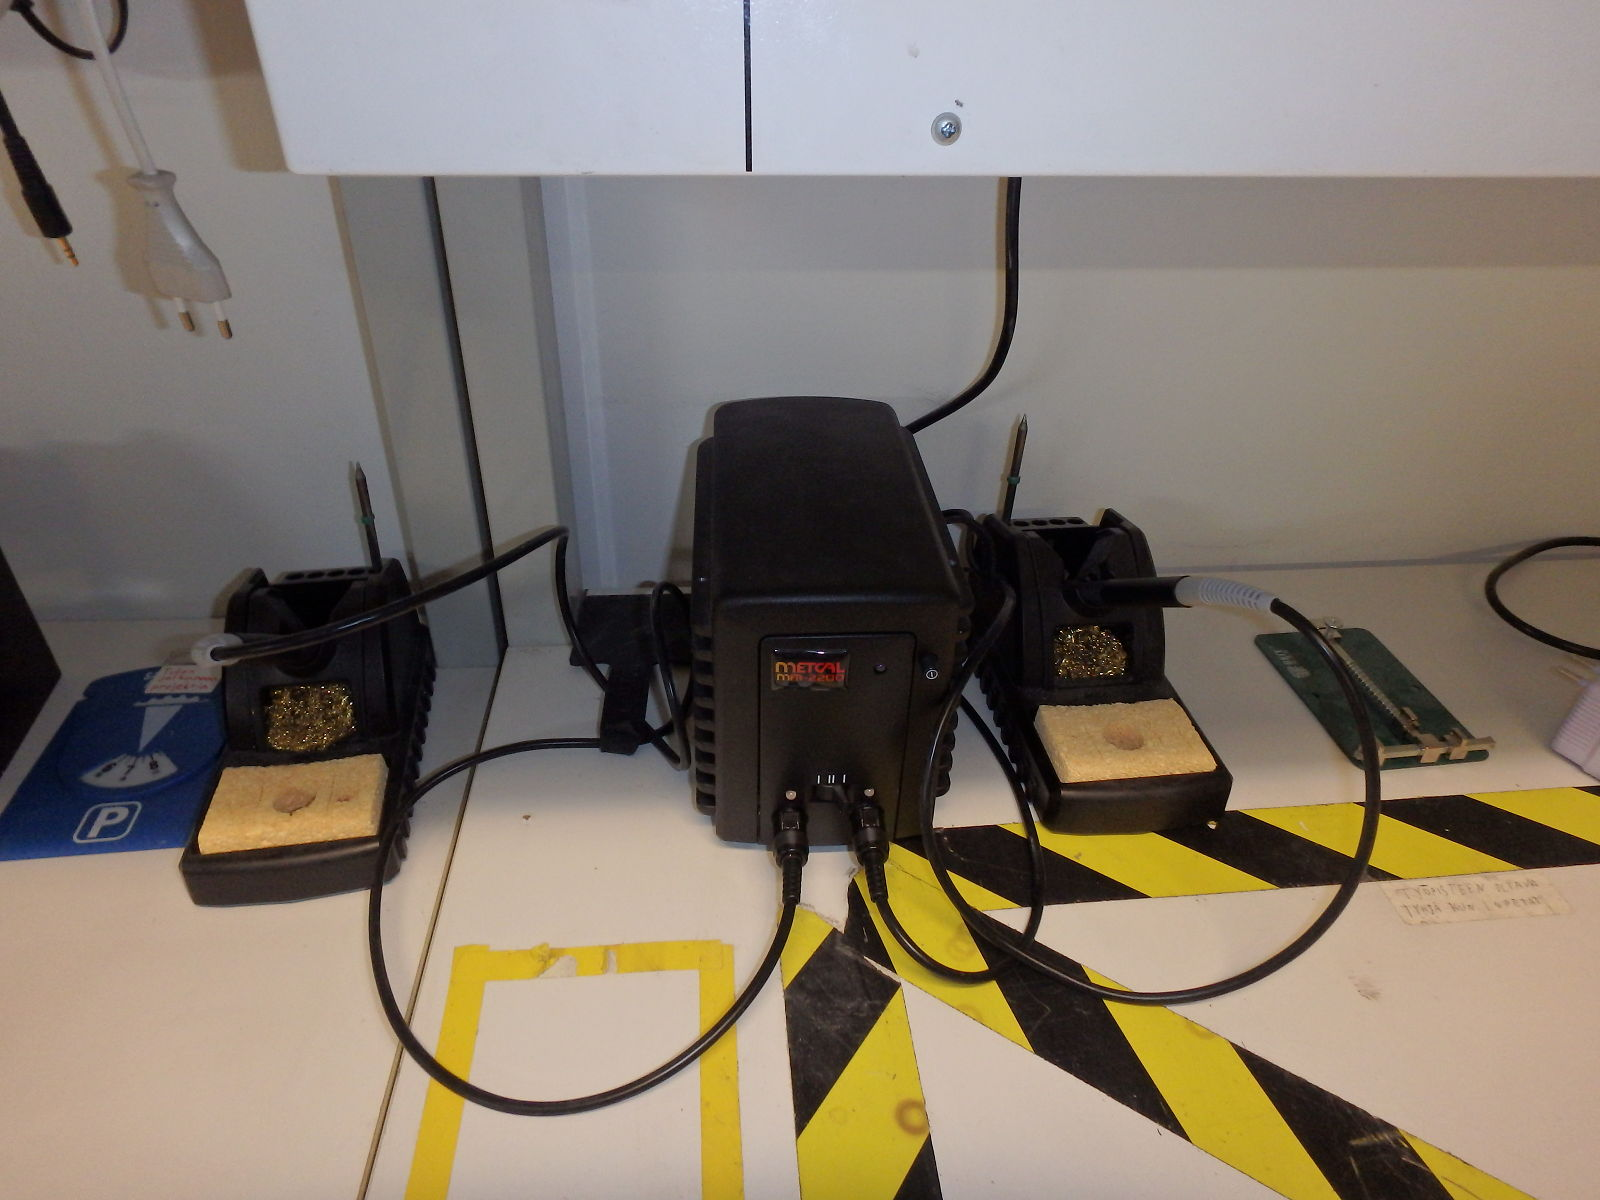
\includegraphics[height=6cm]{images/mfr2200.jpg}
  \end{center}
  \caption{\label{img:mfr2200} Juotosasema}
\end{figure}

L\"amp\"otila s\"a\"atyy automaattisesti k\"arjen mukaan. K\"arkien nimen toinen  kirjain ilmoittaa l\"amp\"otilan:

\begin{table}[htb]
%% Taulukon teksti
\caption{\label{tbl:tip_naming_scheme_temp} K\"arkien l\"amp\"otila \cite[p. 32]{MetcalTips}}
\begin{center}
\fbox{
\begin{tabular}{l l l}
\textbf{Nimi (SxV)} & \textbf{L\"amp\"otila} & \\ \hline
T = temperature sensitive      & 365 \degree C \\ \hline
F = FR4 / Glass Fiber      & 421 \degree C \\ \hline
C = Ceramic      & 460 \degree C \\ \hline
\end{tabular}
}
\end{center}
\end{table}

K\"ayt\"oss\"amme on T- ja F-sarjan k\"arki\"a. Suosittelemme T-sarjan k\"arkien k\"aytt\"amist\"a, F-sarjan k\"arjet on tarkoitettu l\"ahinn\"a lyijytt\"omien juotosten tekemiseen. K\"arjet erottaa toisistaan helposti, F-sarjan k\"arjiss\"a on vihre\"a rengas. 

K\"arki vaihdetaan kytkem\"all\"a kyseinen kolvi pois p\"a\"alt\"a, toista voi k\"aytt\"a\"a vaihdon aikana. Ota kolvin johtoon kytketyll\"a alustalla k\"arjest\"a kiinni ja ved\"a k\"arki ulos. Laita k\"arki kolvin telineen takana olevaan pitimeen ja ty\"onn\"a uusi k\"arki syv\"alle kolviin.

P\"oyd\"an alla on Metcalin k\"aryimuri BVX-200 \cite{MetcalBVX200}. Juottamisessa syntyv\"at k\"aryt ovat terveydelle vaarallisia, etenkin jos k\"ayt\"at fluxia ja kuumaa kolvin k\"arke\"a. Imurin saa p\"a\"alle painamalla juotosaseman vieress\"a olevaa vihre\"a\"a nappulaa. Imu tulee p\"oyd\"an reunoihin kiinnitetyist\"a k\"asivarsista. K\"asivarren voi taivuttaa ty\"oskentelyalueelle. 

\begin{figure}[htb]
  \begin{center}
    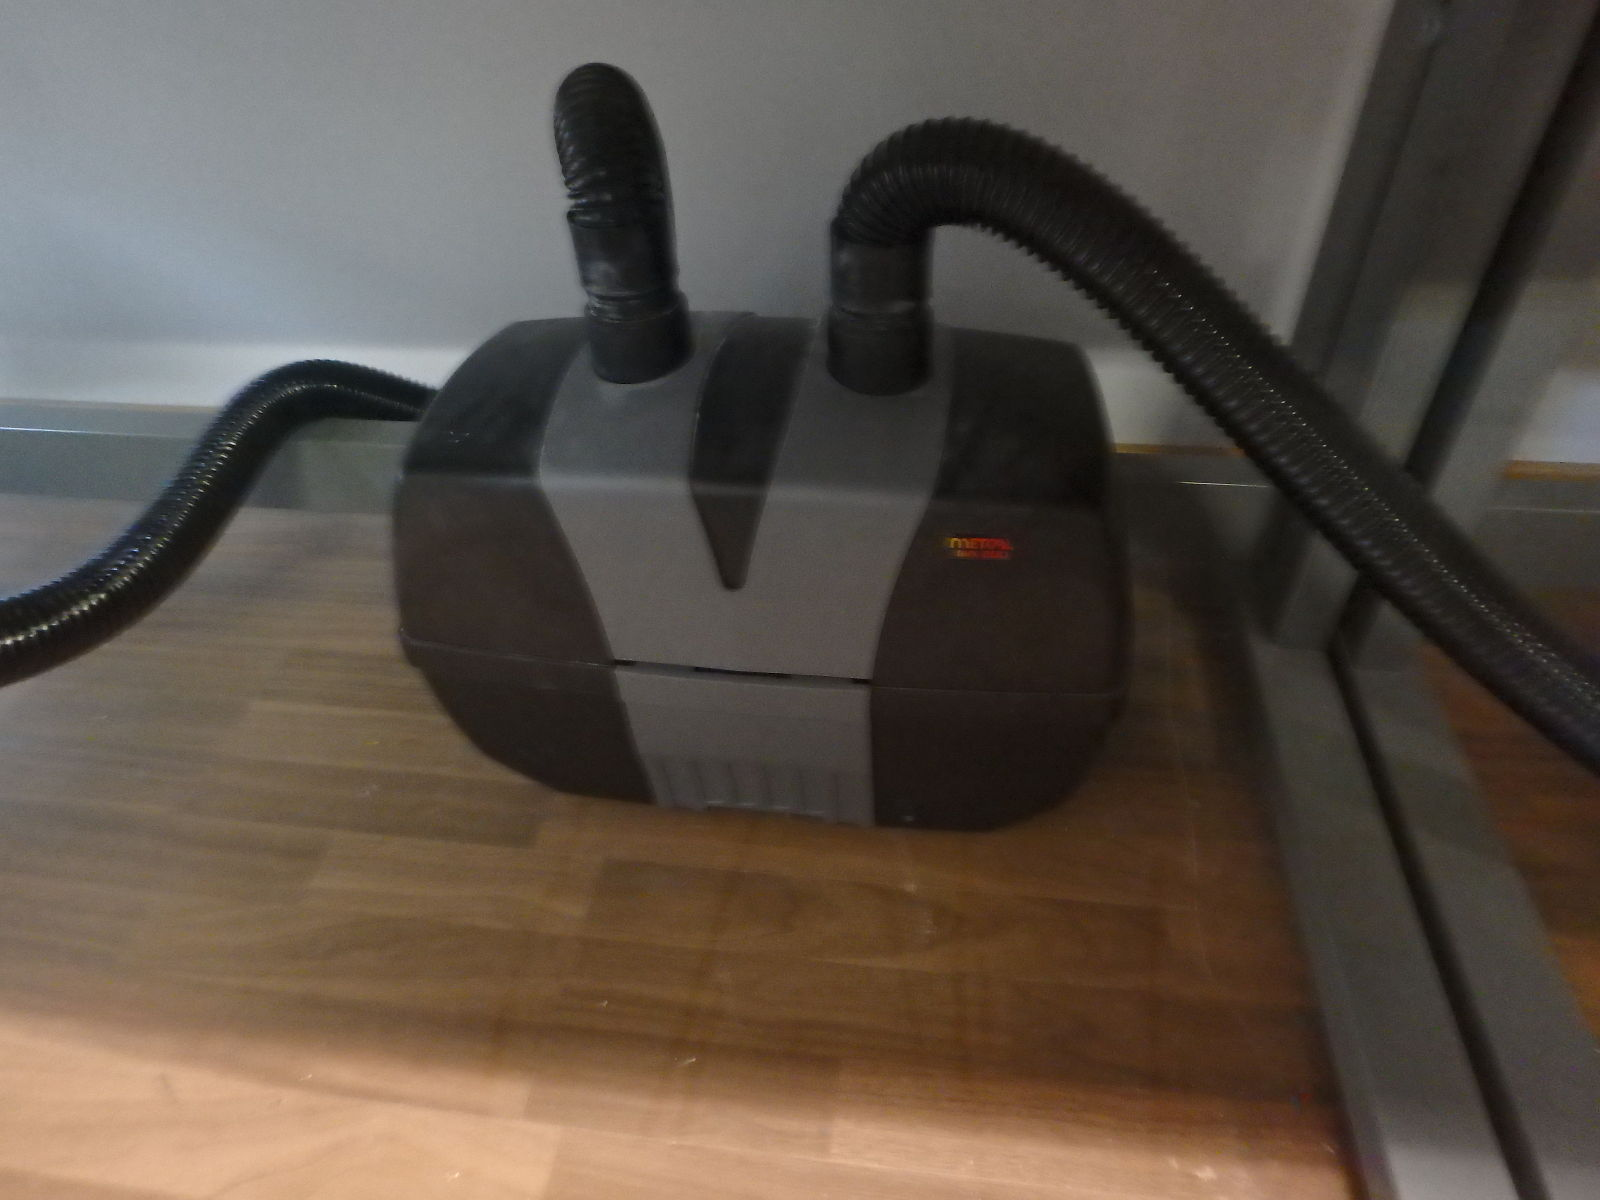
\includegraphics[height=6cm]{images/bvx200.jpg}
  \end{center}
  \caption{\label{img:fume_extractor} K\"aryimuri}
\end{figure}

\section{Vikatilanteet}
Jos kolvi ei l\"ampi\"a, tarkista n\"am\"a kohdat Wirallisesta Ohjekirjasta \cite[p. 3]{MetcalInstructions}. 

\begin{table}[htb]
%% Taulukon teksti
\caption{\label{tbl:troubleshooting} Vianetsint\"a \cite[p. 32]{MetcalTips}}
\begin{center}
\fbox{
\begin{tabular}{l l l}
\textbf{Tilanne} & \textbf{Korjaus} & \\ \hline
Virtaled on punainen.      & Kytke kolvi maadoitettuun pistorasiaan. \degree C \\ \hline
Kolvin led on punainen      & Aseta k\"arki kolvin pohjalle.  \degree C \\ \hline
Kolvin led on yh\"a edelleen punainen      & K\"arki on rikki. Ilmoita asiasta s\"ahk\"opostitse tilavastaavalle. \degree C \\ \hline
K\"aryimuri ei k\"aynnisty      & Varmista ett\"a imurin kotelossa oleva virtan\"app\"ain on asennossa 1 \\ \hline
\end{tabular}
}
\end{center}
\end{table}

\phantomsection
\addcontentsline{toc}{section}{\refname}
%\addcontentsline{toc}{section}{References}
\bibliography{library}
\bibliographystyle{plain}

\vfill

\LaTeX 
\end{document}

